Between the plethora of algorithms used to approximate the solutions of the protein folding problem, one of the most promising is Reinforcement Learning.

\subsection{Basics of Reinforcement Learning} \label{BRL}

RL is a kind of algorithm that is particularly effective when the program is able to interact with the analyzed system.
The main structure of a RL algorithm is that of an \emph{agent} which interacts with an \emph{environment} and on the base of its actions gets as feedback a \emph{reward} and the new state of the environment.
The goal of the model is to find the best \emph{policy} which is a function that returns the action that maximizes the reward at each state.


\begin{figure}[H]
    \centering
    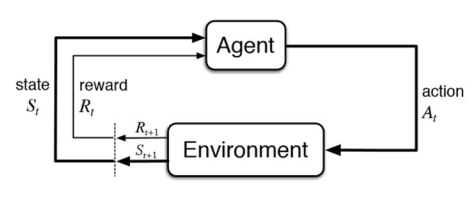
\includegraphics[width=.75\textwidth]{img/rl0.png}
    \caption{Basic architecture of a Reinforcement Learning algorithm}
    \label{fig:rl0}
\end{figure}

\subsubsection{Markov Decision Processes}

MDPs are at the core of RL algorithms, since they describe a discrete-time stochastic control process.
The name comes from the fact that they are an extension of the Markov chains, which are systems in which the evolution of a state depends only on the current state and not on its past. (For more on the topic \cite{bellman1957markovian})


It is then necessary to describe in Markov terms fig \ref{fig:rl0}.
\emph{S} is the set of all possible states and \emph{A} is the set of all possible actions.
The distribution of all possible rewards \emph{R}, can be obtained by every couple of states and actions (s, a) and for each possible adjacent couple of states there is a transition probability \emph{P} associated.

In the following paragraph we will use a common notation in RL which is that of using the capital letters to denote sets and the lowercase ones to denote single elements of the set

\subsubsection{Choosing optimal policies}

For each discrete instant t the system moves from a state $s_{0}$ to a state $s_{1}$ choosing an action $a$. After each action the agent receives a reward $r$. 
In order to choose the optimal policy the algorithm must maximize the cumulative reward starting from a state $s_{0}$, defined as: 
\begin{equation}
\pi^{opt} = \max\left\{E\left(\sum_{t>0}r^{t*r|\pi}\right)\right\}
\end{equation}
It is worth mentioning that the expectation value has an additional constant called discount factor ($\gamma$).
The expectation value for a single trajectory takes the form: $E(r) = r_{0} + \gamma r_{1} + \gamma^{2} r_{2} + \ldots$.
From this expression it is clear that the role of the discount factor is that of giving more weight to closer rewards. This is justified due to intrinsic uncertainty that future rewards hold as a part of an MDP.

To choose in which way the algorithm should try to reach the optimal policy, the designer can choose between two different approaches:

\begin{itemize}
    \item learning through \emph{State Value} function: this function returns the sum of all rewards received starting from an input state following a fixed policy.
        Using this function one can choose the best route through states
    \item learning through \emph{Action Value} function: this function returns the expected reward of taking a given action at a given state.
        If an algorithm uses the action value function it's called a \emph{Q-learning} algorithm    
\end{itemize}

\subsubsection{Q-Learning} \label{Qlearning}

Q-learning is an extremely useful tool to solve the problem of non-deterministic MDPs.
The algorithm exploits the Q-function to associate to each state action pair a scalar value (\emph{Q-values}).
Q-values are defined as the sum of all discounted rewards assuming the Agent is in state s and performs action a, and then continues playing until the end of the episode following some policy $\pi$.
An optimal Q-value is a Q-value that follows the optimal policy. All Q-values are stored in the so called \emph{Q-table}.

\subsubsection{Bellman Equation and Optimal Q-values}

The Bellman equation for Q-learning gives the conditions for equilibrium at correct Q-values, setting therefore a constraint to optimize the policy.
\begin{equation}
Q(s_{0}, a) = r(s_{0},a ) + \gamma  \max_{a'}\left\{Q(s_1, a')\right\}
\end{equation}
$Q(s_{0}, a)$ is the Q-value associated with the couple ($s_{0}$, $a$), $r(s_{0},a )$ is the reward associated with the same couple and the term $\gamma \max_{a'}\left\{Q(s_1, a')\right\}$ is the discounted maximum Q-value for the state-action pair at the successive instant.

\subsubsection{General Q-learning algorithm} \label{GQL}

Q-learning algorithms follow more or less the same general structure
\begin{itemize}
    \item For each pair $(s, a)$ initialize $Q(s, a)$ to 0.
    \item Repeat for each episode (complete iteration that stops at the terminal state)
    \item Select the initial state $s$.
    \item Choose a from s using policy derived from $Q$
    \item Repeat (for each step of the episode)
    \item Take action $a$, observe $r$, $s_{0}$ 
    \item Update table entry: $$Q(s,a) \leftarrow r(s,a) + \gamma \max_{a_{0}}\left\{Q(s_{0},a_{0})\right\}$$
    \item $s \rightarrow{} s_{1}$ until new $s$ is terminal
    \item Until the maximum number of episodes reached or the Q-values do not change
\end{itemize}

An additional parameter might be given to fix how fast the Q-values should change for each iteration.
This parameter is called the \emph{Learning Rate} $\alpha \in [0,1]$. In this case the Bellman equation becomes:
\begin{equation}
Q(s_{0}, a) = (1-\alpha)Q(s_{0}, a) + \alpha \left(r(s_{0},a ) + \gamma  \max_{a'}\left\{Q(s_1, a')\right\}\right) 
\end{equation}

\subsection{Reinforcement Learning applied to the HP model}
The model described is able to solve bidimensional folds for a protein approximated with the HP model.
Its general structure can be generalized to tridimensional folds with very few adjustments, making it a useful tool suited for this specific problem.
This model was first proposed by \cite{czibula2011reinforcement}.

Consider a protein s in the k-dimentional HP model $$s = \left(s_1, \ldots, s_k\right) \ , \ s_i \in \left\{H, P\right\} \ \ \forall i \in \left[1,\ldots,k\right]$$ in order to use RL to solve the problem we need to specify the various components of the RL algorithm: state space, action space, transition function and reward function.

The state space \emph{S} (the agent's environment) is made of $\frac{4^{k}-1}{3}$ elements.
A state is terminal (the process stops) if the number of state visited is $k-1$, so we expect it to visit each possible state. 

The action space \emph{A} is four dimensional and sanctions that from each state the system can transition between four other states (Up, Down, Right, Left or $a_{0}, a_{1}, a_{2}, a_{3}$).

The transition function $\delta$ returns the stochastic outcomes of taking each action in a specific state.
So for each state is given the accessible sequences.
$\delta$ is defined as:
\begin{equation} \label{delta}
\delta(s_{i},a{l})=s_{4 \dot i - 3 + l} \ \ \ l \in [1, 4] \ \ \ \forall i \in \left[1,\frac{4^{k}-1}{3}\right]
\end{equation}
Since there is no reason for initial bias between states the neighbors are all equiprobable with probability of transition $\frac{1}{4}$.

Before defining the reward function it is appropriate to spend a few words to visualize how the RL algorithm described so far models the protein and its folds.
Consider a complete episode and its associated the path $\varsigma = (\varsigma_{0}, \varsigma_1, \ldots , \varsigma_{k-1}) \ \ \varsigma_{i}$.
To this path there will be an action sequence associated $a_{\varsigma} = (a_{\varsigma_{0}}, a_{\varsigma_{1}}, \ldots , a_{\varsigma_{k-2}})$.
This sequence of actions is linked to the path since each element of both sequences appears in equation \ref{delta}.
$a_{\varsigma}$ can be viewed as a possible bidimensional structure of the protein sequence.
Therefore, we can now associate to a certain action sequence, and by extension to a path $\varsigma$, the energy defined in section \ref{sec:model}. 

We can now define the reward function $r(\varsigma_{n}|s_{1}, \varsigma_{1}, \ldots, \varsigma_{l-1})$:
\begin{itemize}
    \item if $a_{\varsigma}$ is not valid $\rightarrow$ 0.01
    \item if the system reached a terminal state $(l = k-1)$ $\rightarrow$ -E
    \item otherwise (``most common case'') $\rightarrow$ 0.1
\end{itemize}
By defining the reward function in this way, it returns the reward received by the agent in the state $\varsigma_{l}$ after it had visited all the previous states.
With the reward function it is now clear that the goal of maximizing the rewards on a path from the starting state to the terminal one is equivalent of that of finding self-avoiding random walks that minimize the associated energy.

\begin{figure}[H]
    \centering
    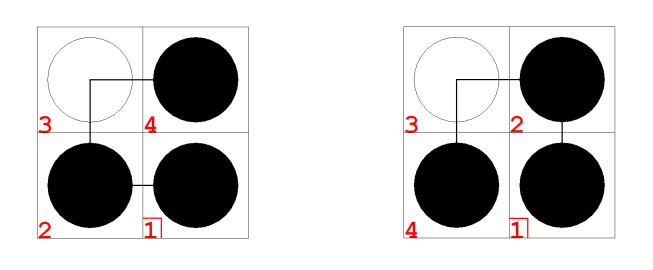
\includegraphics[width=.75\textwidth]{img/rl1.png}
    \caption{Visualization of the link between actions and configuration. In the figure on the right the actions are: Up, Left, Down. In the figure on the right the actions are: Left, Up, Right} \cite{czibula2011reinforcement}
    \label{fig:rl0}
\end{figure}
\subsection{Learning Phase}

For learning it is convenient to use Q-learning. It can be proven that during the training process the values of the Q-table converge to the true values (for the proof see \cite{czibula2011reinforcement}), so it is guaranteed that at the end of the training process the values found will be close to the true values.
After the training the agent acts with a greedy mechanism until it reaches a solution. The adjective \emph{greedy} in this context means that at each step the system transitions to a neighbour state with maximum Q-value.

It is now important to notice that this process might produce more than one optimal policies. In this case, as far as the bidimensional folding goes, the predicted structures will have the same free energy.

\subsection{Beyond Reinforcement Learning}

From what seen so far in this section Q-learning looks like a good way to approach protein folding in the HP model approximation. Despite this, simple Q-learning algorithms such as the one described in section \ref{GQL} are inadequate compared to the state of the art model.

\subsubsection{Deep Q-Learning}

The subject of \emph{Deep Q-learning} is far too complicated and wide to be treated to its full extend in this article, therefore this section contains only its intuitive idea and the main reasons why it ouperforms simple Q-learning.

As we have seen in section \ref{Qlearning} a Q-learning algorithm learns through the process of optimizing the Q-values, which are the best action for a given state given all the previous actions. Deep Q-learning exploits the Neural Networks to estimate cluster of Q-values. In this case there no longer is a Q-table, but a Deep Neural Network estimating many Q-values at the same time, saving resources. 

Since Deep Neural Networks are currently the best statistical estimators available, this kind of algorithm performs extremely well. The price to pay for such improvements is that Deep Neural Networks operate as \textit{black boxes}, meaning that it is often impossible to understand the optimization process for complex problems such as this one

\begin{figure}[H]
    \centering
    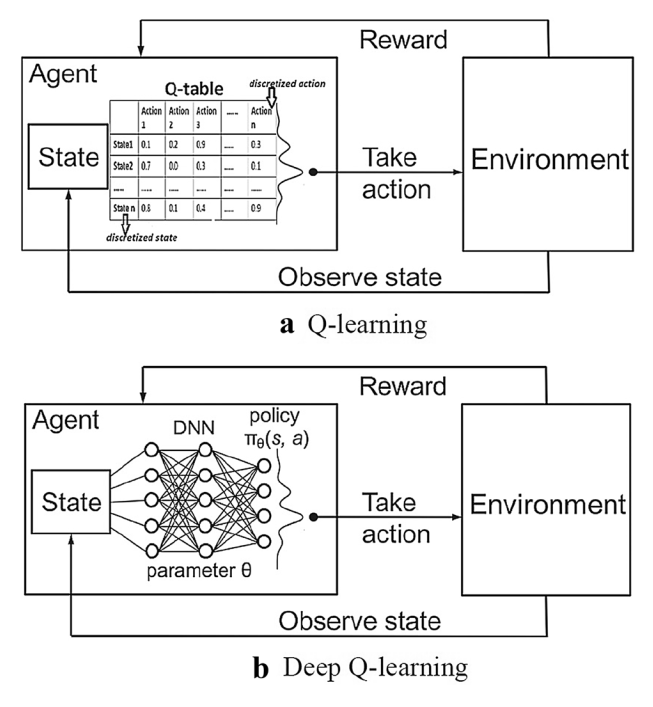
\includegraphics[width=.75\textwidth]{img/rl2.png}
    \caption{Difference between Q-learning and Deep Q-learning visualized \cite{jafari2020solving}
    \label{fig:rl2}
\end{figure}a
